\documentclass[a4paper,UKenglish]{lipics-v2016}
%This is a template for producing LIPIcs articles. 
%See lipics-manual.pdf for further information.
%for A4 paper format use option "a4paper", for US-letter use option "letterpaper"
%for british hyphenation rules use option "UKenglish", for american hyphenation rules use option "USenglish"
% for section-numbered lemmas etc., use "numberwithinsect"
 
\usepackage{microtype}%if unwanted, comment out or use option "draft"
\usepackage{caption}
\usepackage{subcaption}
\usepackage{graphicx}
\usepackage{textcomp} % used for degrees celsius
\usepackage{booktabs}
\usepackage{paralist} % inparaenum support
\usepackage{varioref} % added by Viliam for \vref
\usepackage{xcolor} % added by Viliam for \textcolor
%\usepackage[british]{babel}

% ==========================================
% Custom commands (by Viliam)
% ==========================================
\newcommand{\FOCAL}[3]{ % usage: \FOCAL{R}{M}{op}
  \ifmmode
    #1{\stackrel{\mathtt{#3}}{\circ}}#2
  \else
    \begin{math}\FOCAL{#1}{#2}{#3}\end{math}
  \fi
}
\newcommand{\SOHUP}{
  \ifmmode
    SoH^\uparrow
  \else
  \begin{math}\SOHUP\end{math}
  \fi
}
\newcommand{\SOHDOWN}{
  \ifmmode
    SoH^\downarrow
  \else
  \begin{math}\SOHDOWN\end{math}
  \fi
}
% ==========================================



%\graphicspath{{./graphics/}}%helpful if your graphic files are in another directory

\bibliographystyle{plainurl}% the recommended bibstyle

% Author macros::begin %%%%%%%%%%%%%%%%%%%%%%%%%%%%%%%%%%%%%%%%%%%%%%%%
\title{Vision Paper: Efficient Spatio-Temporal Geo-Statistics for Exploratory Data Analysis}
%\footnote{A full version of the paper is available at \cite{DBLP:journals/cacm/Knuth74}, \url{XXX}}}
\titlerunning{Efficient Spatio-Temporal Geo-Statistics} %optional, in case that the title is too long; the running title should fit into the top page column

%% Please provide for each author the \author and \affil macro, even when authors have the same affiliation, i.e. for each author there needs to be the  \author and \affil macros
\author[1]{Julian Bruns}
\author[1]{Joan R. Access}
\affil[1]{GIScience Research Group, Institute of Geography, Heidelberg University, Heidelberg, Germany\\
  \texttt{firstname.lastname@uni-heidelberg.de}}

\authorrunning{J.\,Q. Open and J.\,R. Access} %mandatory. First: Use abbreviated first/middle names. Second (only in severe cases): Use first author plus 'et. al.'

\Copyright{John Q. Open and Joan R. Access}%mandatory, please use full first names. LIPIcs license is "CC-BY";  http://creativecommons.org/licenses/by/3.0/

\subjclass{Dummy classification -- please refer to \url{http://www.acm.org/about/class/ccs98-html}}% mandatory: Please choose ACM 1998 classifications from http://www.acm.org/about/class/ccs98-html . E.g., cite as "F.1.1 Models of Computation". 
\keywords{Dummy keyword -- please provide 1--5 keywords}% mandatory: Please provide 1-5 keywords
% Author macros::end %%%%%%%%%%%%%%%%%%%%%%%%%%%%%%%%%%%%%%%%%%%%%%%%%

%Editor-only macros:: begin (do not touch as author)%%%%%%%%%%%%%%%%%%%%%%%%%%%%%%%%%%
\EventEditors{John Q. Open and Joan R. Acces}
\EventNoEds{2}
\EventLongTitle{42nd Conference on Very Important Topics (CVIT 2016)}
\EventShortTitle{CVIT 2016}
\EventAcronym{CVIT}
\EventYear{2016}
\EventDate{December 24--27, 2016}
\EventLocation{Little Whinging, United Kingdom}
\EventLogo{}
\SeriesVolume{42}
\ArticleNo{23}
% Editor-only macros::end %%%%%%%%%%%%%%%%%%%%%%%%%%%%%%%%%%%%%%%%%%%%%%%

\begin{document}

\maketitle



\begin{abstract}
Hot spot analysis is essential for geo-statistics.

\end{abstract}


\section{Introduction and Related Work}
The goal of hotspot analysis is the detection and identification of interesting areas. It achieves this goal by computing statistically significant deviations from the mean value of a given study area. This allows a decision maker to easily identify those areas of interest and allows further focus in sub-sequential data analysis or the decision focus. Typical applications range from crime detection over identification of disease outbreaks to urban heat islands. In such applications, scarce resources are then often applied in only those identified hotspots or used as the basis for the allocation. The general approach is an unsupervised learning method similar to a cluster analysis. 

Huge in increase in data, e.g. even without incorporating spatial structures the OSM\cite{OpenStreetMap} data, as example for VGI, is over 1 TB


\subsection{Examples}


Spatio-temporal sentiment hotspot detection using geotagged photos \cite{Zhu:2016:SSH:2996913.2996978}

A framework for evacuation hotspot detection after large scale disasters using location data from smartphones: case study of Kumamoto earthquake \cite {Yabe:2016:FEH:2996913.2997014} :



\cite{Wiener:2016:BCR:2996913.2996931} BigGIS Vision Paper

\cite{7129542} The era of big spatial data : 
"Unfortunately, the urgent need to manage and analyze big
spatial data is hampered by the lack of specialized systems,
techniques, and algorithms to support such data." "We
provide general guidelines to show the four components that
are needed in a system for big spatial data." 
In general an overview of approaches in 2015 and overall targets for systems

\cite{mehta2016spatio}   Spatio-Temporal Hotspot Computation on Apache Spark (GIS Cup) 

Giscup 2016 \footnote{http://sigspatial2016.sigspatial.org/giscup2016/home}

\section{State of the Art}
\subsection{Geostatistic}
While the standard hot spot analysis approaches allow for a fast and automated exploratory analysis of spatial data sets, they are highly dependent on their parametrizations and underlying data. This is quite similar to the challenges in clustering, in particular for the well-known k-means, first coined in \cite{macqueen1967some}, or DBScan (\cite{ester1996density}) algorithm. This leads to an instability of the analysis results, which are then difficult to use with high certainty. Here, a selection of approaches and discussions of the last 15 years are presented how to tackle this instability.

The most general approach is to pre-determine and calculate spatial dependencies, based on the a-priori knowledge of the analyst, the empirical data set or best-practices from previous, similar analyses. A good example for this approach can be found in \cite{suomi2012effects}. In their work, the authors examine the effects of scale on temperature and in particular urban heat island modeling. The pre-determined range of spatial influences is called \emph{buffer zones}; these buffer zones indicate the range of impact in an inner-city temperature measurement scenario. They found that for their empirical data set a buffer zone of 1000m provides the best results. This is familiar to the well-known approach to solve the inherent problem of DBScan, the determination of its distance: OPTICS (\cite{ankerst1999optics}). The disadvantage of this approach is that it has to be manually pre-determined, which results in similar problems as the semi-supervised methods to detect points of interest. It can not be done automatically without introducing an element of uncertainty, which is opposed to our goal to create a more stable approach.

An automated approach is presented with the \emph{A Multidirectional Optimal Ecotope-Based Algorithm} (AMOEBA) in \cite{aldstadt2006using}. The idea behind this approach is to automatically create the optimal, scale-invariant weight matrix and then use this weight matrix in conjunction with a clustering approach to create a graphical overview map of areas of interest. The term ecotope is used for this areas, which is the technical term from the field of biology for the habitat of species. The result is a consistent identification of spatial clusters on a map. In their work they use the $G^*$ statistic as the underlying statistic. The clustering approach is quite similar to DBScan in its approach of creating ecotopes. 


A true modification of the $G^*$ statistic is presented in a later work (\cite{getis2010constructing}) of the same authors called the LSM (local statistics model). They base their modification on the Kriging approach and its ability to model the spatial autocorrelation as a function dependent on the distance. The idea is to model the weight matrix W as a function of the spatial autocorrelation, where each entry of the matrix is a value derived from the empirical  (semi-)variogram. This leads to continuous values up to the so called \emph{critical distance}, which is "defined as the distance beyond which no discernible increase in clustering exist" (\cite{getis2010constructing}). They compare their configuration to other, well-known spatial configuration approaches for the weight matrix W. These are taken from \cite{griffith1996some} and in the words of \cite{getis2010constructing}:
''Research on W has been reviewed by Griffith (1996, p. 80), who concludes that five rules of thumb aid in the specification of weights matrices: 
\begin{enumerate}
\item “It is better to posit some reasonable geographic weights matrix than to assume independence.” This implies that one should search for or theorize about an appropriate W and that better results are obtained when distance is taken into account.
\item “It is best to use surface partitioning that falls somewhere between a regular square and a regular hexagonal tessellation.” Griffith suggests that for planar data, a specification between four and six neighbors is better than something either above six or below four. Of course, the configuration of the planar tessellations will play a role here (\cite{boots2000global}).
\item “A relatively large number of spatial units should be employed, n > 60.” Following from the law of large numbers, most spatial research, especially due to unequal size spatial units, would require fairly large samples.
\item “Low-order spatial models should be given preference over higher-order ones.” Following from the scientific principle of parsimony, it is always wise to choose less complicated models when the opportunity presents itself.
\item “In general, it is better to apply a somewhat under-specified (fewer neighbors) rather than an over-specified (extra neighbors) weights matrix.” \cite{florax1995impacts} found this result by identifying the power of tests. Overspecification reduces power. They recognize that “Uncertainty with respect to proper specification has long been recognized as a fundamental problem in applied spatial econometric modeling” (p. 132).
\end{enumerate}
''

\cite{ord2001testing} discuss the question in how to formulate the $G^*$ statistic to focus more on local pattern, while still accounting for the global autocorrelation. They propose the $O$ statistic which uses the (semi-)variogram to subdivide the data set into several '' 'relatively homogeneous' subregions'' (\cite{ord2001testing}). This allows the identification of smaller, more local hot spots, which can be overshadowed in bigger data sets. Finally, they restrict the general applicability in that the version presented in their work requires spatial stationarity.

\cite{westerholt2015local} present a scale-sensitive version of the local $G^*$ statistic, which they call the \emph{GS statistic}. The motivation for this modification is to account for the differences in the scale (the impact of the area under investigation) of the data set, i.e. whether a data set includes only the inner city or also its surrounding area. The problem lies in the detection and use of the local context of the gathered data. A fixed weight matrix W does not include the difference in context, e.g. in Twitter feeds. Their approach is to redefine the neighborhood of a data point with upper and lower distance thresholds, which are then used in pairwise comparisons. Only sufficiently connected data points within their thresholds are considered to be viable as a hot spot and only those points are used for the global mean and global deviation values. They evaluated their approach on Twitter data of the city of San Francisco, USA and show that this leads to reduction or even negation of cross-scale interference. The main restrictions of this approach lies in its increased computational costs as well as its reliance on continuous distance functions.


For futher literature regarding the creation of optimal weight matrices for spatial associations we refer to the work of \cite{aldstadt2006using}, where they provide an exhaustive overview of the state of the art.

\cite{Bruns2017} for focal $G^*$ and efficient parametrization of $G^*$

\subsection{Frameworks and Methods}
An Effective High-Performance Multiway Spatial Join Algorithm with Spark \cite{ijgi6040096}
"In this paper, we present an effective
high-performance multiway spatial join algorithm with Spark (MSJS) to overcome the multiway
spatial join bottleneck." "Spatial analysis is the core engine that drives research and applications of GIS."


GeoSpark: a cluster computing framework for processing large-scale spatial data \cite{Yu:2015:GCC:2820783.2820860}

Spatio-Temporal Join on Apache Spark \cite{Whitman:2017:SJA:3139958.3139963}

Algorithmically-Guided User Interaction \cite{vanDijk:2017:AUI:3139958.3140032}

GeoMesa: a distributed architecture for spatio-temporal fusion \cite{hughes2015geomesa}

geotrellis\footnote{https://geotrellis.io/}

\section{Vision}

\section{Challenges}

\section{Conclusion}






\subsection{Hot Spot Analysis}
The goal of hotspot analysis is the detection of interesting areas as well as patterns in spatial information. One of the most fundamental approach is Moran´s I~\cite{MoranI}. There it is tested whether or
not a spatial dependency exists. This gives the information on global
dependencies in a data set. Upon this hypothesis test several geo-statistical
tests are based. The most well known are the Getis-Ord statistic~\cite{Ord.1995}
and LISA~\cite{Anselin.1995}. In both cases the general, the global statistic of
Moran´s I is applied in a local context. The goal is to detect not only global
values, but instead to focus on local hotspots and to measure the significance
of those local areas. 

Existing methods for determining hot spots are dependent on the parametrization
of the weight matrix as well as on the size of the study area. Intuitively,
increasing the size of a weight matrix has a "blurring" effect on the raster
(




\section{Evaluation}

\subsection{Dataset}

We evaluate our data on the New York city yellow cab data set 
\footnote{$http://www.nyc.gov/html/tlc/html/about/trip\_record\_data.shtml$}. 
This data set includes all taxi drives from the yellow cabs in New York City, 
from location, to passengers and many more informations. In this study, we compare the 
total pickups over January from 2016 in the Manhattan area. 
The borders of the rasters are (40.699607 \textdegree  (N), -74.020265 \textdegree  (E)) 
and (40.769239 \textdegree  (N), -73.948286 \textdegree  (E)) after WGS84.
By using this data set, we reduce the computational effort while still 
being able to show the applicability on real world data and problems.
\subsection{Treatments}



\begin{figure*}[htp]
  \centering

  \vspace{1em}
  \begin{tabular}{cccccccc}
    \multicolumn{8}{l}{G* computed using different weight matrix sizes} \\
    \hline
    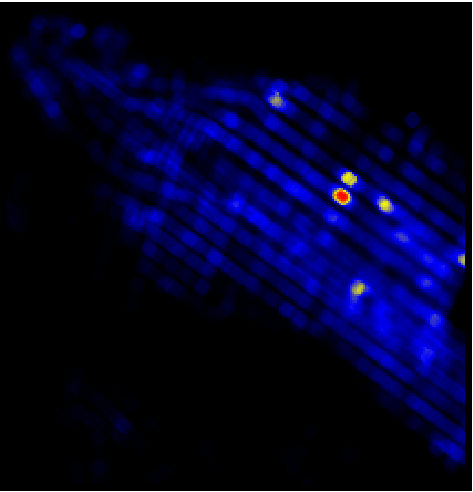
\includegraphics[width=4.6em]{images/gen-raw-blur-gstar-1}&
    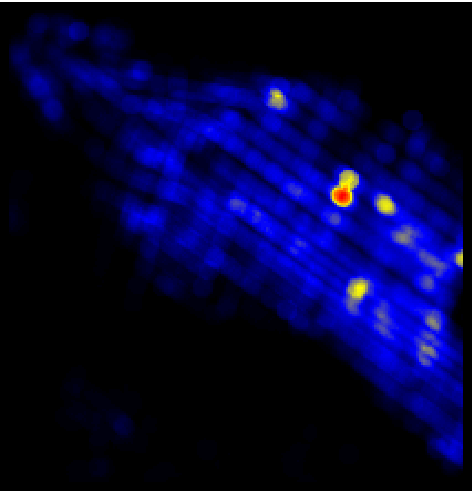
\includegraphics[width=4.6em]{images/gen-raw-blur-gstar-2}&
    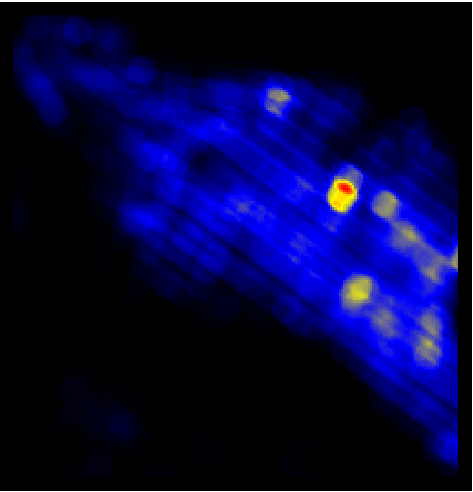
\includegraphics[width=4.6em]{images/gen-raw-blur-gstar-3}&
    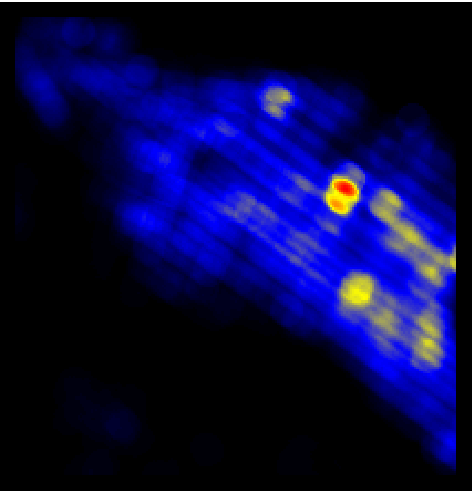
\includegraphics[width=4.6em]{images/gen-raw-blur-gstar-4}&
    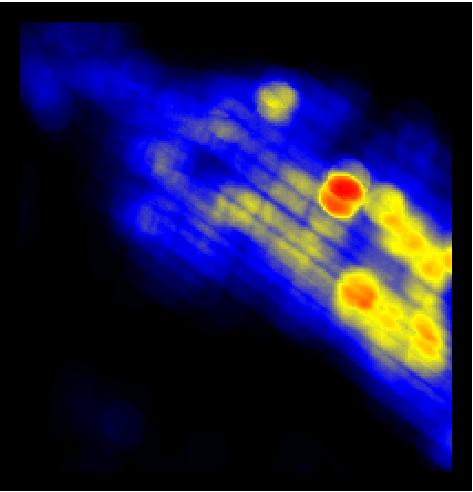
\includegraphics[width=4.6em]{images/gen-raw-blur-gstar-5}&
    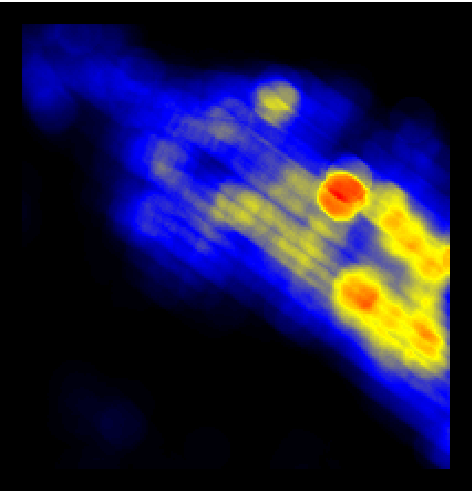
\includegraphics[width=4.6em]{images/gen-raw-blur-gstar-6}&
    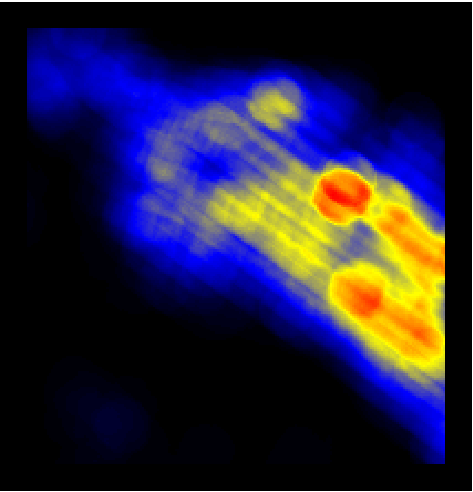
\includegraphics[width=4.6em]{images/gen-raw-blur-gstar-7}&
    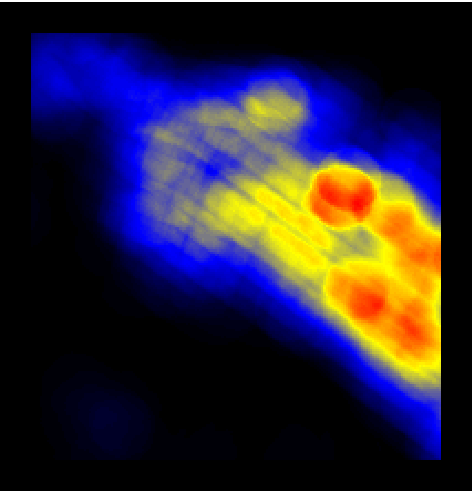
\includegraphics[width=4.6em]{images/gen-raw-blur-gstar-8}\\
    
    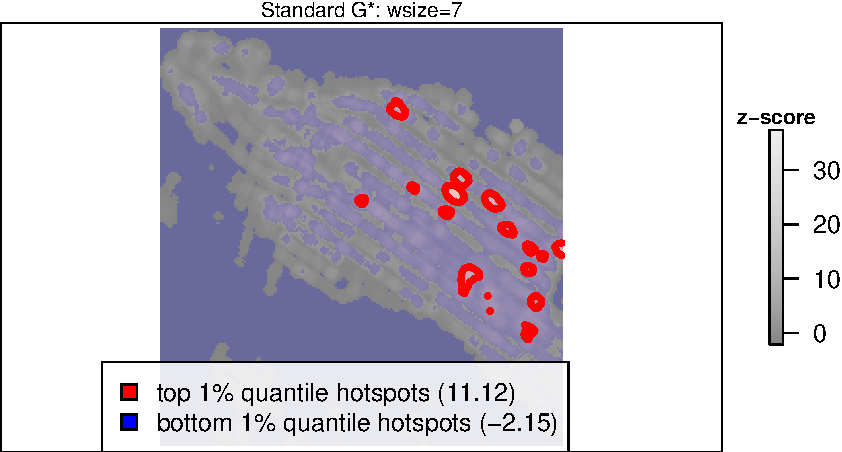
\includegraphics[width=4.6em]{images/gen-demo-blur-gstar-1}&
    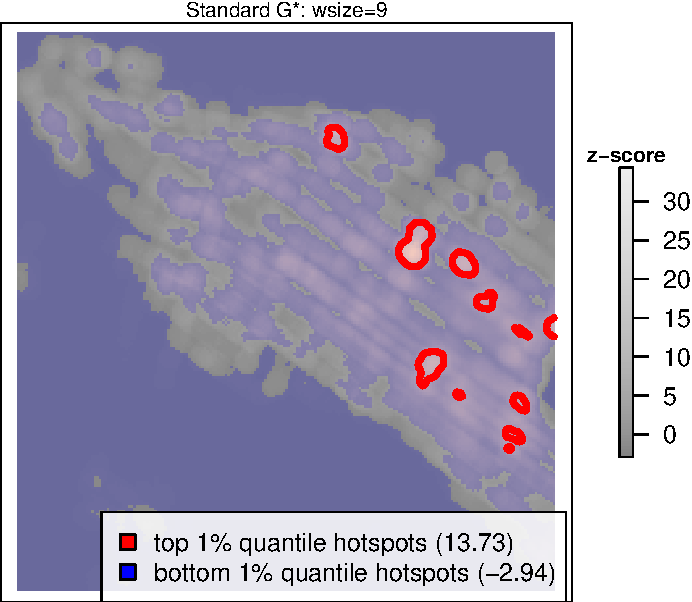
\includegraphics[width=4.6em]{images/gen-demo-blur-gstar-2}&
    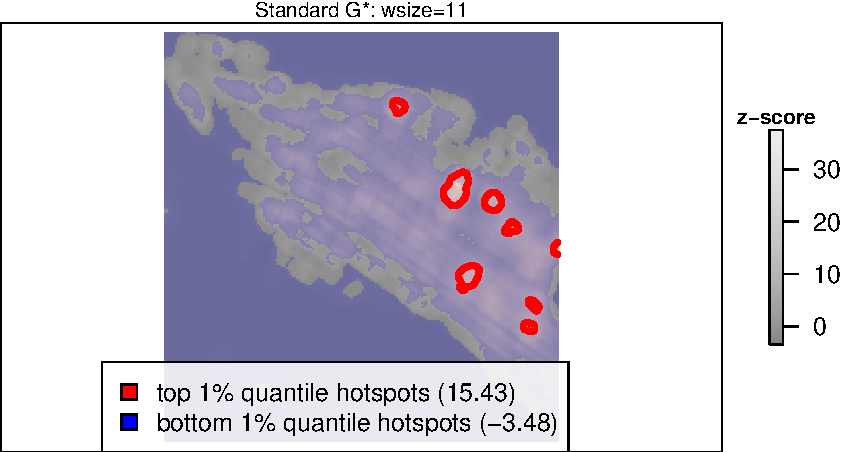
\includegraphics[width=4.6em]{images/gen-demo-blur-gstar-3}&
    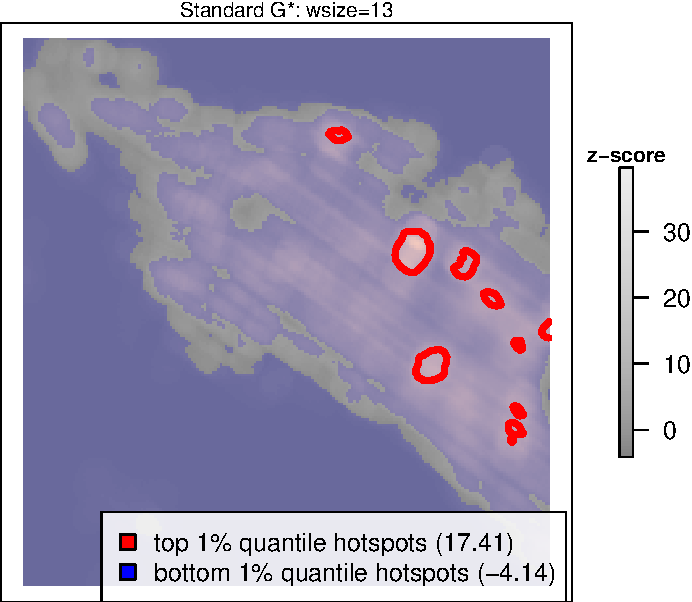
\includegraphics[width=4.6em]{images/gen-demo-blur-gstar-4}&
    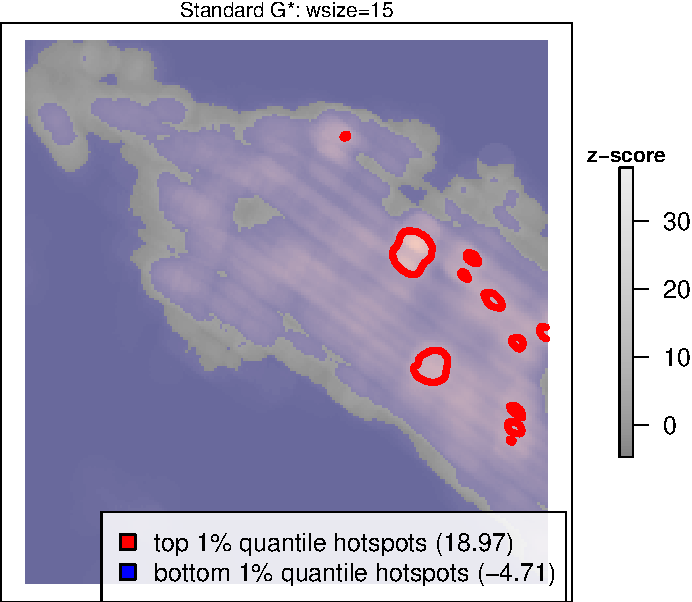
\includegraphics[width=4.6em]{images/gen-demo-blur-gstar-5}&
    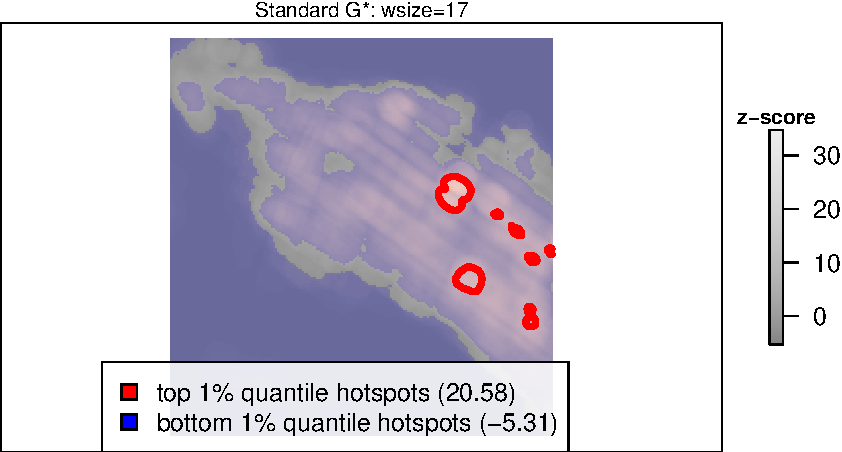
\includegraphics[width=4.6em]{images/gen-demo-blur-gstar-6}&
    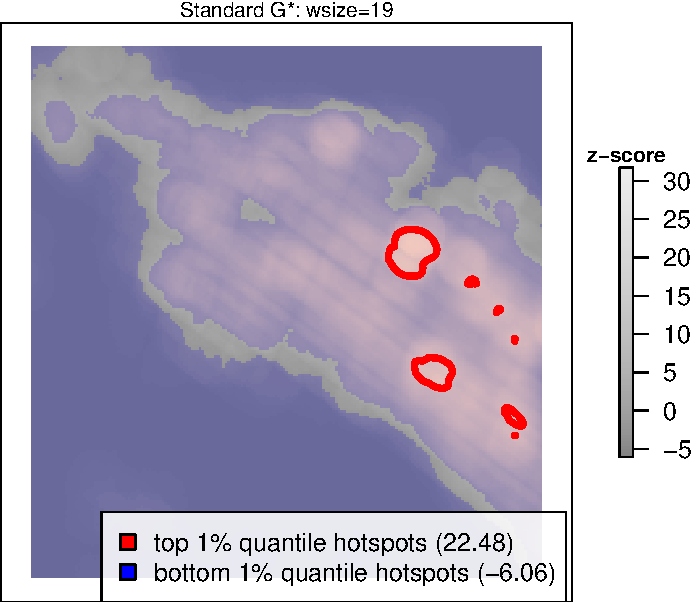
\includegraphics[width=4.6em]{images/gen-demo-blur-gstar-7}&
    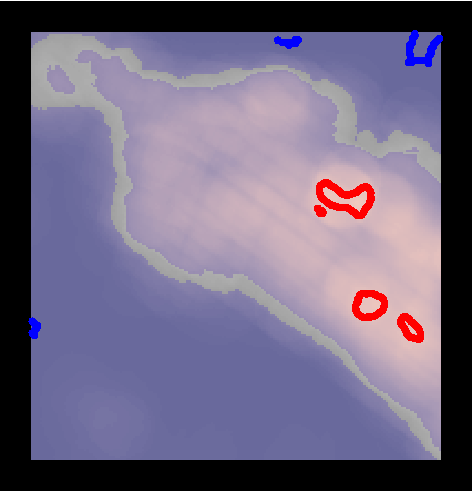
\includegraphics[width=4.6em]{images/gen-demo-blur-gstar-8}\\
  \end{tabular}


  \caption{
    This image shows different weight matrix sizes for G* and Focal G* together 
    with two metrics -- $SoH^\uparrow$ and $SoH^\downarrow$.
  }
  \label{fig:Blur}
\end{figure*}


\bibliography{references}


\end{document}
